\subsection{Kommunikation von Dateien innerhalb der Serveranwendung}
Alle Attribute, Parameter und Rückgaben, die im Entwurfsheft mit dem Typ \glqq File\grqq{} gekennzeichnet waren, haben wir jetzt als Path implementiert. Wobei wir die Klasse Path aus dem Modul pathlib der Python-Standardbibliothek importieren.

Im Folgenden soll die Handhabung der Dateien unter Zuhilfenahme von Pfaden erklärt werden. Dateien, die durch die API die oberste Schicht der Serverandwendung erreichen werden zunächst in einem temporären Ordner zwischengespeichert. Der entsprechende Pfad im temporären Ordner wird entweder durch Aufruf eines Konstruktors in einem Objekt abgelegt oder unmittelbar an die Schnittstelle des Workflow-Packages übergeben.
Dort wird der Datei dann ein langfristiger Speicherort im Dateisystem zugewiesen. Die Löschung der Dateien im temporären Ordner obliegt dem Empfänger. 

Muss umgekehrt eine Datei vom Workflow-Package an die Schnittstelle der Serveranwendung gealngen, so wird der Pfad des langfristigen Speicherorts verwendet. Dort kann die Datei ausgelesen werden, gelöscht wird sie anschließend natürlich nicht.

Im Entwurfsheft haben wir uns keine Gedanken über die Ordnerstruktur der auf dem Server gespeicherten Dateien gemacht, deshalb reichen wir nun einen entsprechenden Entwurf nach. 

\begin{figure}[h]
            \label{ordnerstruktur}
            \centerline{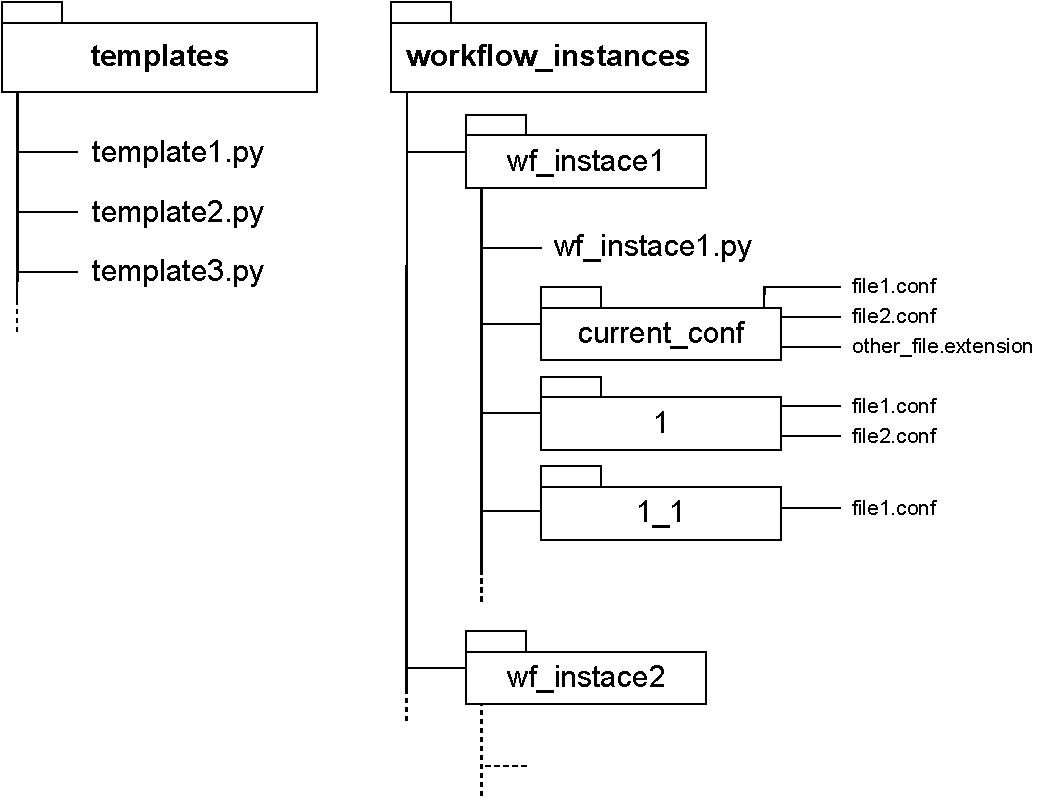
\includegraphics[scale=0.7]{res/ordnerstruktur.pdf}}
            \caption{Eine graphische Veranschaulichung der Ordnerstruktur}
\end{figure}

Zum einen gibt es den Ordner \glqq templates\grqq{}, der unmittelbar alle Dag-definition-files der bisher erstellten Templates enthält. Der Name der Datei stimmt dabei stets mit dem Namen des Templates überein. 

Daneben gibt es zudem noch den Ordner \glqq workflow\_instances\grqq{}. Dieser enthält für jede erstellte Workflow-Instanz einen Unterordner, der den eindeutigen Namen der Instanz trägt. 

In jedem dieser Unterordner befinden sich mindestens die Dag-Definition-File der Instanz und der Ordner \glqq current\_conf\grqq{}, der in seiner Struktur stehts dem ursprünglich Konfigurationsordner enspricht. Insbesondere können auch Dateien mit einer Endung darin liegen, die nicht \glqq.conf\grqq{} ist. Die \glqq .conf\grqq{}-Dateien sind dabei immer auf dem Stand der aktuellen Version der Workflowinstanz. 

Ebenfalls fester Bestandteil ist der Ordner \glqq 1\grqq{}, der die initiale Version der Instanz representiert. In ihm liegen alle \glqq.conf\grqq{}-Dateien in ihrer ursprünglichen Fassung. Zusätzlich gibt es noch für jede neu erstellte Version einen Ordner, in dem stets nur die in dieser Version geänderten \glqq.conf \grqq{}-Dateien liegen.

\subsection{Änderungen im Workflow-Package}

\begin{figure}[h]
            \label{workflow_klassen}
            \centerline{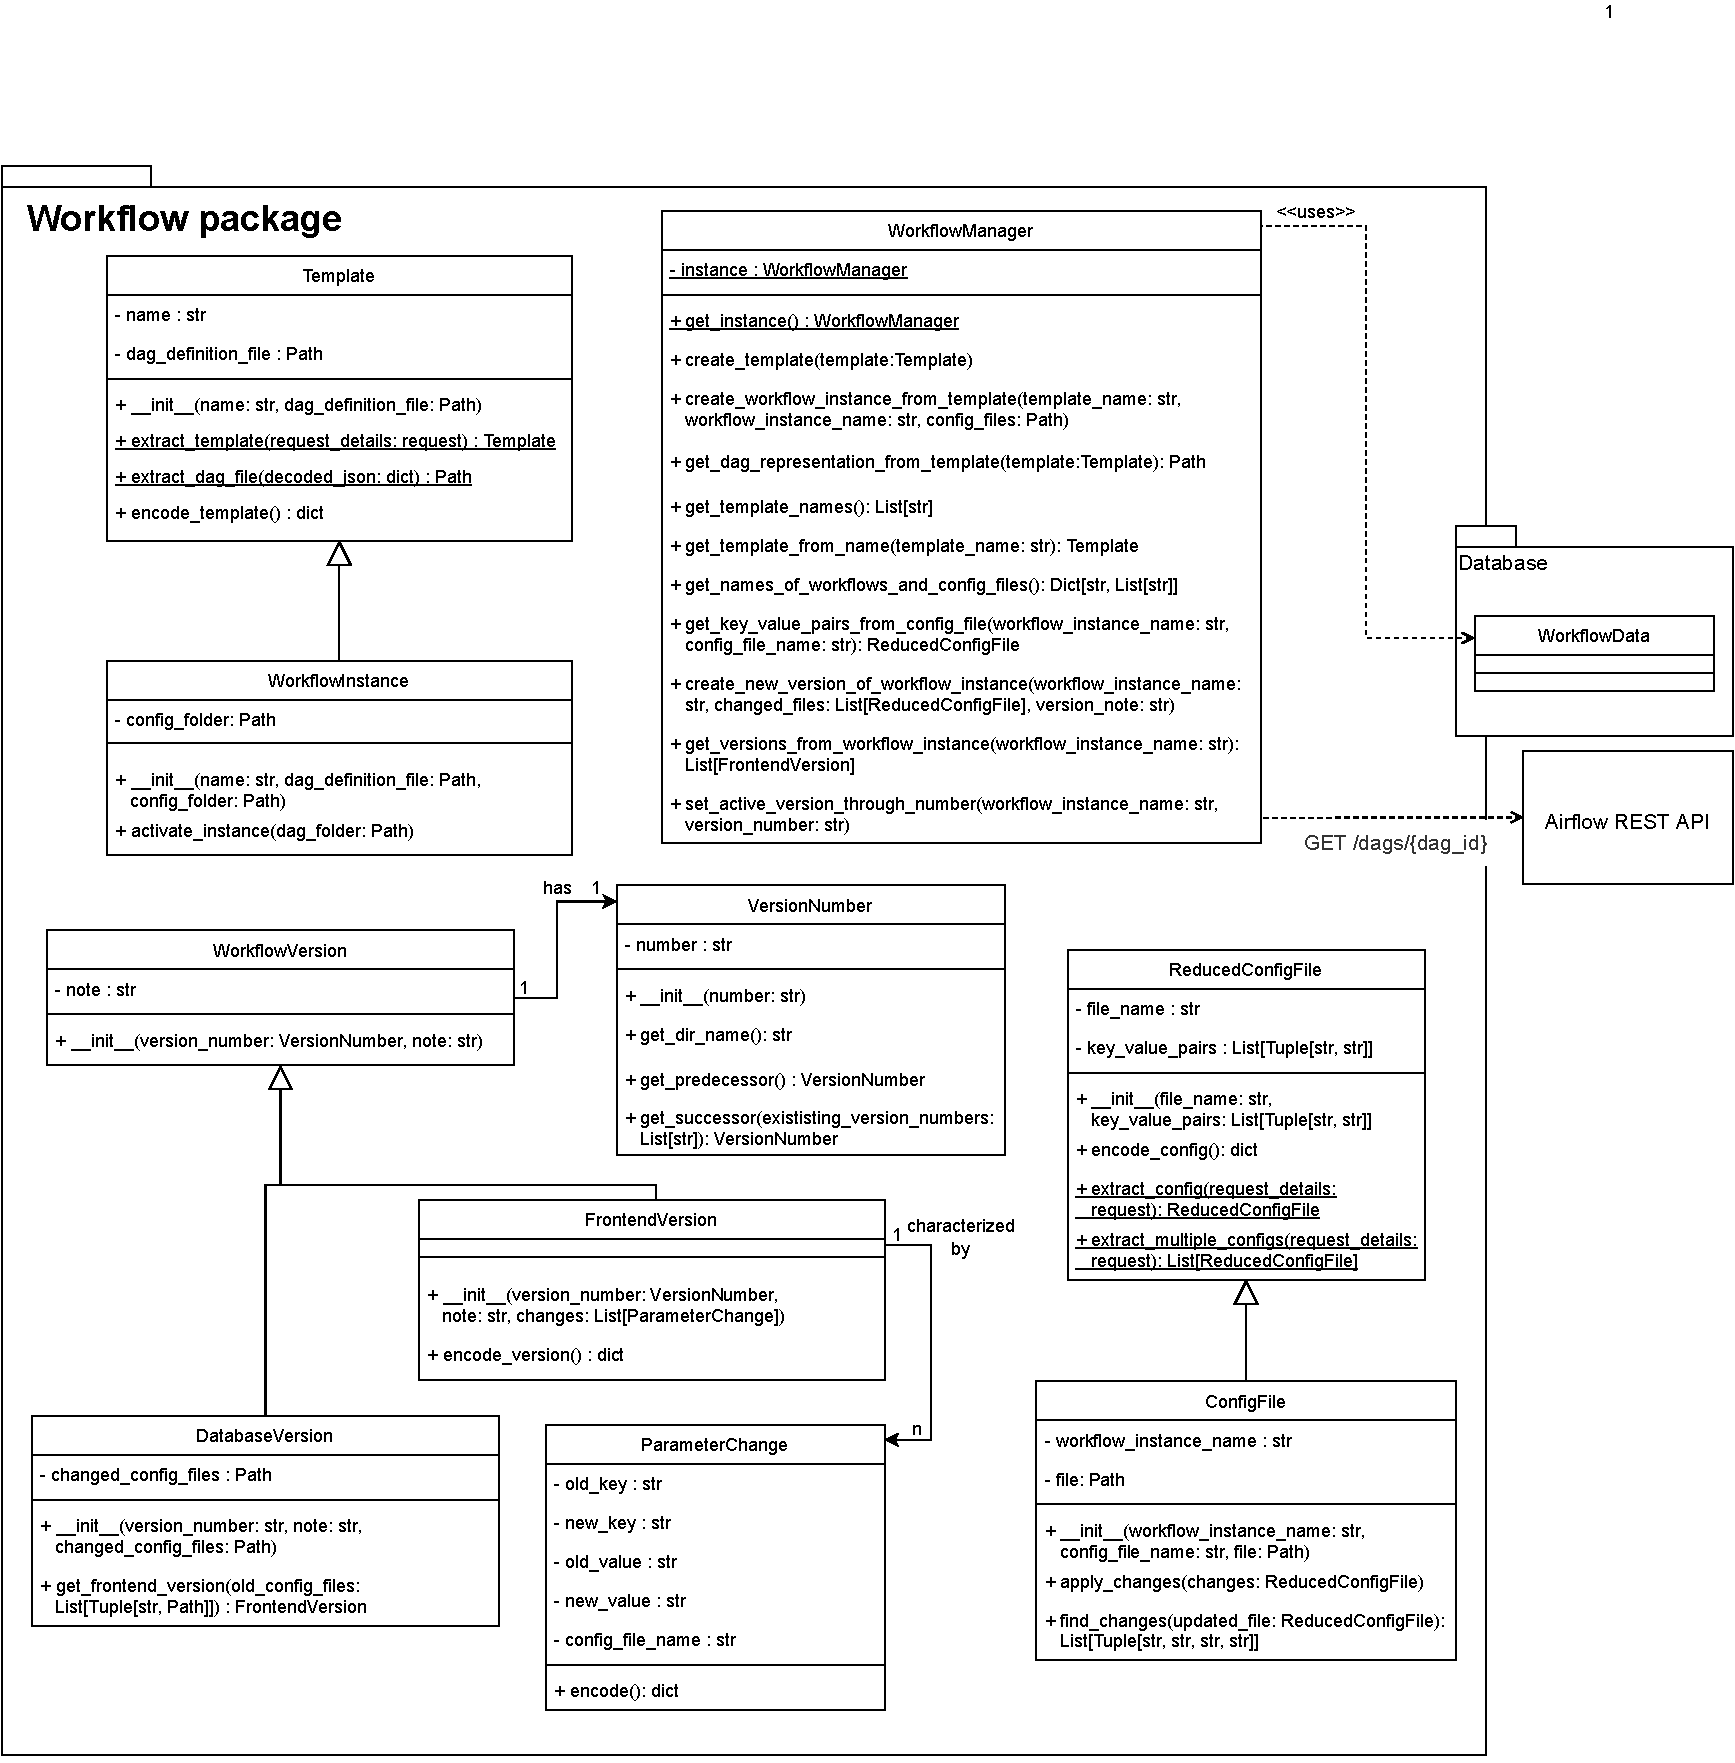
\includegraphics[scale=0.5]{res/workflow_class_diag.pdf}}
            \caption{Das überarbeitete Klassendiagramm des Workflow Packages}
\end{figure}

\begin{description}
\item[Ersetzung von Arrays durch Listen]\hfill \\
An allen Stellen in denen im Entwurf ein Array vorgesehen war. Haben wir in der Implementierung Listen verwendet. Der wichtigste Grund dafür ist, dass Python die Verwendung von Listen schlicht besser unterstützt. Die Syntax die Python für den Umgang mit Listen anbietet erhöht dabei auch die Lesbarkeit des Programmcodes. Abstriche in der Performanz sind nicht zu erwarten, weil davon auszugehen ist, dass die Anzahl der Listenelemente sich in moderaten Bereichen bewegt.
\item[Rückgabetyp von get\_names\_of\_workflows\_and\_config\_files in WorkflowManager]\hfill
Das Informationsbedürfnis, das diese Methode abdecken soll sind für alle Workflow-Instanzen der Name und die Namen aller \glqq .conf\grqq{}-Dateien der Instanz. Das ursprüngliche Format war, für jede Instanz eine Liste von Strings, die zunächst den Namen der Instanz gefolgt von den Namen der Dateien enthalten sollte. Beim Implementieren kamen wir dann aber auf die wesentlich elegantere Lösung Dictionarys zu verwenden. Dabei sind die Namen der Instanzen Schlüssel und die Liste Namen der Dateien die zugehörigen Werte.
\item[Umbenennung der Klasse Version in WorkflowVersion]\hfill \\
Durch die Umbenennung ist klar, dass es die Workflow-Instanzen sind, die versioniert werden.
\item[Verwefen der statischen Methode from\_string in VersionNumber]\hfill \\
Die Methode entpuppte sich als überflüssig, da sie sich zur stark mit dem Konstruktor überschnitt. Dieser hat als einzigen Eingabeparameter auch einen String. Die Prüfung ob der String dem Format einer Versionsnummer entspricht kann ebenfalls direkt im Konstruktor erfolgen.
\item[En- und Decode-Methoden in den Datenklassen]\hfill \\
Die Begründung und Details zu dieser Änderung finden sich in \ref{json_backend}.
\item[Neue Methode get\_frontend\_version in DatabaseVersion]\label{get_f_version}\hfill \\
In der neue Methode berechnen die Versionen mit ihren veränderten Dateien unter Hinzugabe der vorherigen Dateien, die Unterschiede zur Vorgänger-Version. Ursprünglich lag diese Funktionalität in der WorkflowManager-Klasse. Da das DatabaseVersion-Objekt aber selbst alle Informationen besitzt um die Berechnung durchzuführen, wäre es eine Missachtung des Kapselungsprinzips sie auf einer höheren Ebene anzusiedeln.
\item[Verwefen der Attribute active\_version und version\_numbers in der Klasse WorkflowInstance] \hfill
Die Klasse WorkflowInstance kommt nur bei der Erstellung von Instanzen zum Einsatz. Da zu diesem Zeitpunkt aber immer nur die Version \glqq 1\grqq{} existiert, kamen die oben genannten Attribute nie zum Einsatz.
\item[Neue Methode activate\_instance in WorkflowInstance]\hfill \\
Sehr ähnlich wie bei der Methode get\_frontend\_version handelt es sich auch hier um Funktionalität die vom WorkflowManager in eine tiefere Ebene verschoben wurde. Die Methode ist dafür verantwortlich in der Dag-Definition-File den Namen der Instanz als dag\_id einzutragen und die File in den \glqq dags\grqq{}-Ordner von Airflow zu kopieren. Die Methode ist bisher noch nicht implementiert.
\end{description}